% based on a template made by the university of cologne
% http://www.mi.uni-koeln.de/wp-MIEDV/wp-content/uploads/2016/07/LaTeX-Vorlage.zip - 2023-11-02
\documentclass[12pt,a4paper]{scrartcl}

\addtokomafont{sectioning}{\rmfamily}
\usepackage[ngerman]{babel}% deutsches Sprachpaket wird geladen
\usepackage[T1]{fontenc} % westeuropäische Codierung wird verlangt
\usepackage[utf8]{inputenc}% Umlaute werden erlaubt
\usepackage[usenames]{color} % Erlaubt die Benutzung der namen im Farbpaket und deren Änderung
\usepackage{amsmath} % Erweiterung für den Mathe-Satz
\usepackage{amssymb} % alle Zeichen aus msam und msmb werden dargestellt
\usepackage{graphicx} % Graphiken und Bilder können eingebunden werden
%\usepackage{multirow} % erlaubt in einer Spalte einer Tabelle die Felder in mehreren Zeilen zusammenzufassen
\usepackage{enumerate} % erlaubt Nummerierungen
\usepackage{xurl} % Dient zur Auszeichnung von URLs; setzt die Adresse in Schreibmaschinenschrift.
\usepackage[center]{caption}  % Bildunterschrift wird zentriert
%\usepackage{subfigure} % mehrere Bilder können in einer fugure-Umgebung verwendet werden
%\usepackage{longtable} % Diese Umgebung ist ähnlich definiert wie die tabular-Umgebung, erlaubt jedoch mehrseitige Tabellen.
%\usepackage{paralist} % Modifikation der bereits bestehenden Listenumgebungen
\usepackage{lmodern}% Für die Schrift
\usepackage[hidelinks]{hyperref} % Links und Verweise werden innerhalb von PDF Dokumenten erzeugt
%\usepackage{wrapfig} % Das Paket ermöglicht es von Schrift umflossene Bilder und Tabellen einzufügen.
\usepackage{latexsym} % LaTeX-Symbole werden geladen
\usepackage{tikz} % Erlaubt es mit tikz zu zeichnen
\usepackage{tabularx} % Erlaubt Tabellen
\usepackage{algorithm} % Erlaubt Pseudocode
\usepackage{color} % Farbpaket wird geladen
%\usepackage{stmaryrd} % St Mary Road Symbole werden geladen
\usepackage{physics}
\usepackage[version=4]{mhchem} % Chemie: \ce & \pu

\numberwithin{equation}{section} % Nummerierungen der Gleichungen, die durch equation erstellt werden, sind gebunden an die section
\newcommand{\HRule}{\rule{\linewidth}{0.7mm}}
\newcommand{\code}[1]{\textsf{#1}}

\hypersetup{
  pdftitle={B1.4: Photoelektrischer Effekt},
  pdfcreator={\LaTeX}
}

\setcounter{secnumdepth}{6}
\setcounter{tocdepth}{6}

\begin{document}
\begin{titlepage}
	\pagestyle{empty}

	\begin{center}

	\textsc{\LARGE Universität zu Köln }\\ [0.4cm]
	\textsc{Mathematisch--Naturwissenschaftliche Fakultät} \\[1.5cm]

	
\includegraphics[width=0.45\textwidth]{../media/uni.jpg} \\[1.5cm]  % Uni-Logo wird geladen

	\textsc{\Large Praktikum~B}\\[2mm]
	\textsc{11. Juni 2024}\\[10mm]
	\HRule \\[0.4cm]

		{	\Huge \bfseries B1.4}\\[0.4cm]
			{	\huge \bfseries Photoelektrischer Effekt}\\[0.3cm]
	
	\HRule \\[3cm]

 	\begin{center}
		\textsc{\Large Catherine~Tran } \\[3pt]
		\textsc{\Large Carlo~Kleefisch } \\[3pt]
		\textsc{\Large Oliver~Filla } \\[3pt]
	\end{center}
	\end{center}
\end{titlepage}

\newpage
\tableofcontents
\newpage

\clearpage
\hypertarget{einleitung}{%
\section{Einleitung}\label{einleitung}}

Der photoelektrische Effekt beschreibt die Auslösung von Elektronen aus einem Material, das mit Licht einer bestimmten Frequenz bestrahlt wird. Diese Elektronen haben nach dem Austritt eine kinetische Energie, die von der Frequenz des Lichts abhängt.

Die Energie der Elektronen hängt jedoch nicht von der Intensität des Lichtes ab. Dadurch kann nicht jede elektromagnetische Strahlung für den Photoeffekt verwendet werden. Die Intensität bestimmt stattdessen die Anzahl der Elektronen, die in einer bestimmten Zeit ausgelöst werden und einen Photostrom bilden.

Dieses Phänomen war bereits im 19. Jahrhundert beobachtet worden, konnte jedoch nicht erklärt werden. Ohne die Quantenphysik nahm man an, dass die Energie des Lichts von seiner Amplitude und Intensität abhänge, ähnlich wie bei makroskopischen Wellen. Dies stand jedoch im Widerspruch zum beobachteten Photoeffekt.

\textsc{Albert Einstein} erklärte diesen Effekt im Jahr 1905 durch seine Lichtquantenhypothese. Nach dieser besteht das Licht einer Frequenz $\nu$ aus Quanten mit der Energie $h\nu$. Damit ist der fehlende Zusammenhang von Lichtintensität und kinetischer Energie der Elektronen erklärbar.

\clearpage
\hypertarget{theoretische-grundlagen}{\section{Theoretische Grundlagen}\label{theoretische-grundlagen}}

\subsection{Physikalische Grundlagen}
\subsubsection{Elektrische Felder}
\label{Elektrische Felder}

Das elektrische Feld ist ein Vektorfeld, welches jedem Punkt im Raum den Vektor der elektrischen Feldstärke $\vec{E}$ zuordnet. Diese beschreibt die Coulomb-Kraft $\vec{F}_C$, die auf eine Ladung $Q$ an diesem Ort wirkt.

\begin{eqnarray}
	\vec{E} &=& \frac{\vec{F}_C}{Q}
\end{eqnarray}

\noindent
Feldlinien werden als Darstellungsmittel verwendet und liegen tangential an der Feldstärke $\vec{E}$. Feldlinien beginnen in positiven und enden in negativen Ladungen.

\subsubsection{Spannung}
\label{Spannung}
Um eine elektrische Ladung von einem Ort $A$ zu einem Ort $B$ zu bewegen, muss elektrische Arbeit $W_{AB}$ aufgebracht werden. Sie hängt von der Feldstärke ab.

Die \emph{elektrische Spannung} beschreibt diese Arbeit unabhängig von der zu verschiebenden Ladung $Q$. \cite{Gerthsen}

\begin{eqnarray}
	U_{AB} &=& \frac{W_{AB}}{Q}
\end{eqnarray}

\subsubsection{Transmission von Licht}
Wie jede Welle kann auch Licht ein Medium durchdringen. Der \emph{Transmissionsgrad} $T$ eines Mediums beschreibt, welcher Anteil von einfallender Strahlung transmittiert wird. Er ist der Quotient aus der Beleuchtungsstärke vor dem Medium $I_0$ sowie hinter demselben $I$. \cite{Gerthsen}

\begin{eqnarray}
	T &=& \frac{I}{I_0}
\end{eqnarray}

\noindent
Der Transmissionsgrad eines Mediums hängt im Allgemeinen von der betrachteten Wellenlänge ab. Es gibt verschiedene Filter, um die Strahlungsintensität zu reduzieren.

Ein \emph{Farbfilter} lässt nur Licht einer bestimmten Wellenlänge hindurch. Für diese Wellenlänge beträgt der Transmissionsgrad näherungsweise $1$, für alle anderen Wellenlängen $0$. % Quelle: https://de.wikipedia.org/wiki/Farbfilter

Im Unterschied dazu lässt ein \emph{Graufilter} oder Neutraldichtefilter alle Wellenlängen in gleicher Stärke hindurch. Der Transmissionsgrad ist damit idealerweise unabhängig von der Wellenlänge. % Quelle: https://de.wikipedia.org/wiki/Neutraldichtefilter

\subsubsection{Austrittsarbeit}
Die Austrittsarbeit $W_A$ ist die Energiedifferenz zwischen Fermi--Niveau $E_F$ in einem Material und dem Vakuumniveau mit $E_\mathrm{pot}(\infty)=0$, das dem elektrischen Potential in unendlicher Entfernung entspricht. Da die Fermi--Niveaus materialabhängig sind, trifft dies auch auf die Austrittsarbeit zu. \cite{Demtröder}

\begin{eqnarray}
	W_A &=& E_\mathrm{pot}(\infty) - E_F \\
	W_A &=& -E_F
\end{eqnarray}

\noindent
Das einfachste quantenmechanische Erklärungsmodell ist der Potentialkasten, der in Abbildung \ref{fig:Austrittsarbeit} dargestellt ist.

\begin{figure}[h!]
	\centering
	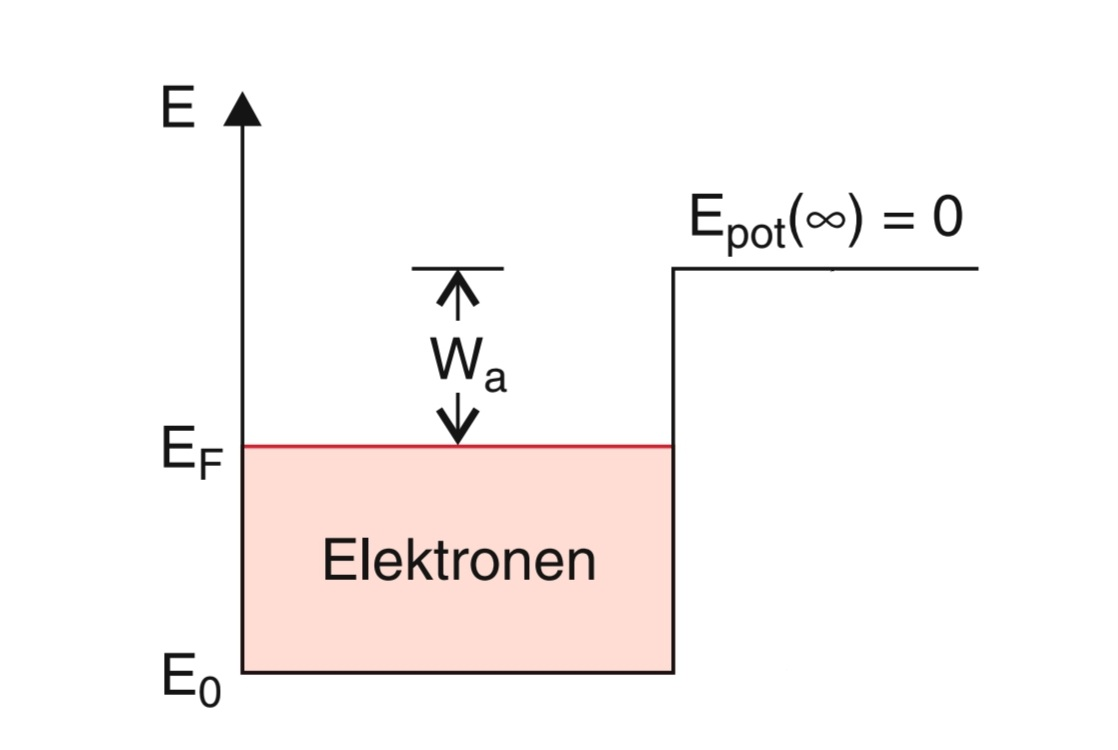
\includegraphics[width=0.5\textwidth]{../media/B1.4/Austrittsarbeit_Potentialkasten.jpg}
	\caption{Austrittsarbeit $W_a$ aus einem Potentialkasten \cite{Demtröder}}
	\label{fig:Austrittsarbeit}
\end{figure}

\subsubsection{Kontaktspannung}
Berühren sich zwei unterschiedliche Metalle mit verschiedenen Austrittsarbeiten, so entsteht eine Spannung an der Kontaktstelle.

Diese \emph{Kontaktspannung} $U_K$ wird durch Elektronen verursacht, die von dem Metall mit der geringeren Austrittsarbeit $W_1$ in das mit der höheren Austrittsarbeit $W_2$ übergehen. Dadurch kommt es zu einem Ladungsungleichgewicht. Dieser Prozess endet in einem Gleichgewichtszustand, wenn $U_K$ der Differenz der Fermi--Niveaus $\Delta E_F$ entspricht.

\begin{eqnarray}
	\Delta E_F &=& e \cdot (\Phi _2 - \Phi _1) \\
		&=& e \cdot U_K \\
	\Delta E_F &=& W_2 - W_1 \\
	\Rightarrow U_K &=& \frac{W_2 -W_1}{e}
\end{eqnarray}

\noindent
In diesem Versuch entspricht $W_2=W_A(A)$ der Austrittsarbeit der Anode, während $W_1=W_A(K)$ die der Kathode beschreibt.

Betrachtet man die Elektronen im Metall als Elektronengas, dann gilt die Boltzmann--Verteilung. Die Kontaktspannung lässt sich aus dem Verhältnis der Elektronenzahldichten $n_1$ und $n_2$ bestimmen. Dabei finden die Boltzmann-Konstante $k_B$, die Temperatur $T$ in Kelvin und die Elementarladung $e$ Verwendung.

\begin{eqnarray}
	U_K &=& \frac{k_B T}{e} \ln \left( \frac{n_2}{n_1} \right) \label{eq:Kontaktspannung}
\end{eqnarray}

\noindent
Aufgrund der dichten Gase muss korrekterweise die Fermi--Verteilung verwendet werden. \cite{Gerthsen} Dies wird jedoch in diesem Versuch vernachlässigt.

\subsubsection{Photoeffekt}
Der \emph{äußere photoelektrische Effekt} beschreibt das Auslösen von Elektronen aus einer Materialoberfläche unter Bestrahlung mit elektromagnetischen Wellen. Dazu muss die Strahlung eine Grenzfrequenz $\nu_g$ aufweisen, deren Energie der Austrittsarbeit entspricht.

Ein Lichtquant mit einer Frequenz $\nu$ besitzt eine Energie $h\nu$, die durch das Planck'sche Wirkungsquantum $h$ beschrieben wird. Aufgrund der Energieerhaltung erhält jedes herausgelöste Elektron eine maximale kinetische Energie $E_\mathrm{max}$.

\begin{eqnarray}
	E_\mathrm{max} &=& h\nu - W_A \\
		&=& \frac{1}{2} m_e v^2 \\
	h &=& 4.135 \cdot 10^{-15} \mathrm{\,eV \cdot s}
\end{eqnarray}

\noindent
Die Grenzfrequenz $\nu_g$ kann durch die Austrittsarbeit $W_A$ der Photokathode bestimmt werden.

\begin{eqnarray}
	\nu_g &=& \frac{W_A}{h}
\end{eqnarray}

\noindent
Der Photoeffekt hängt vollständig von der Frequenz ab, nicht von der Intensität der Strahlung. Bei hoher Intensität werden in einem Zeitrahmen mehr Elektronen herausgelöst. Beträgt die Frequenz weniger als die Grenzfrequenz, findet unabhängig von der Intensität kein äußerer Photoeffekt statt.

Die Austrittsarbeit liegt in der Größenordnung Elektronenvolt, beispielsweise $2.1\mathrm{\,eV}$ (Barium) oder $4.91\mathrm{\,eV}$ (Nickel). \cite{Demtröder} Daher kann Licht im sichtbaren und ultravioletten Spektrum den äußeren Photoeffekt auslösen.

Im \emph{inneren Photoeffekt} werden Elektronen nicht aus dem Material gelöst, sondern aus dem Valenzband in das Leitungsband angeregt. Dieser Prozess kann in Halbleitermaterialien stattfinden.

\subsection{Elektrotechnik}
\subsubsection{Funktionsweise einer Photozelle}
Eine Photozelle besteht aus einer Photokathode und einer Anode in einem Glaskolben, siehe Abbildung \ref{fig:photozelle}.

Fällt Licht auf die Photokathode, so werden durch den Photoeffekt Elektronen aus der Kathode gelöst. Einige dieser sogenannten \textit{Photoelektronen} treffen auf die Anode. Dadurch entsteht ein elektrisches Feld zwischen den Elektroden.

\begin{figure}[h]
	\centering
	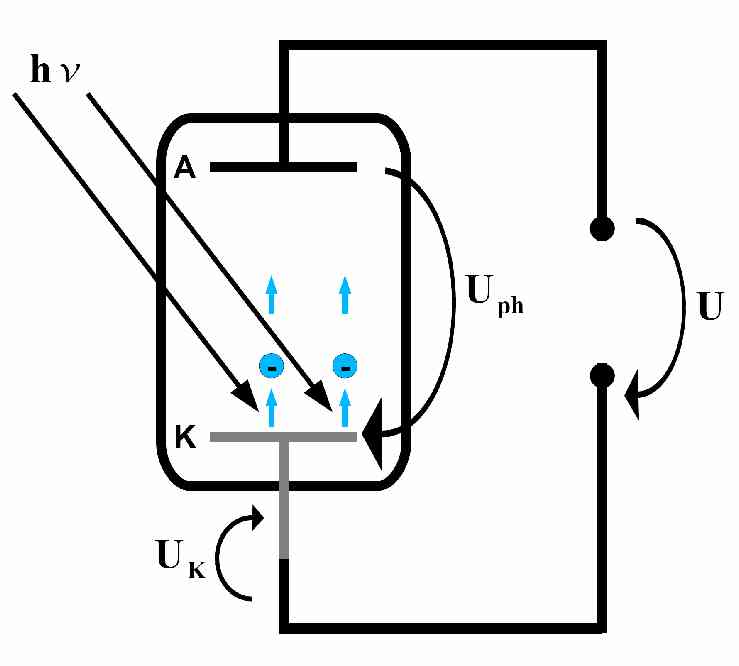
\includegraphics[width=0.4\textwidth]{../media/B1.4/Photozelle.jpg}
	\caption{Darstellung einer Photozelle mit Kathode $K$ und Anode $A$, \\
		mit Stoppspannung $U_\mathrm{Ph}$, Kontaktspannung $U_K$ und messbarer Spannung $U$ \cite{uni}}
	\label{fig:photozelle}
\end{figure}

Die Photoelektronen können auf ihrem Weg zur Anode abgebremst werden, indem eine externe Spannung an den Elektroden angelegt wird. Hierbei muss an der Anode eine negative Spannung angelegt werden.

Die \textit{Stoppspannung} $U_{\mathrm{Ph}, 0}$ ist die minimale Spannung, die alle Photoelektronen abbremst. Sie hängt von der Energie des Lichts $h\nu$ mit Frequenz $\nu$ und der Austrittsarbeit $W_A(K)$ der Kathode ab. \cite{Gerthsen}

\begin{eqnarray}
	e \cdot U_{\mathrm{Ph}, 0} &=& h \cdot \nu - W_A (K) \label{eq:Stoppspannung}
\end{eqnarray}

\noindent
Die Photokathode besteht aus einem Material mit geringer Austrittsarbeit $W_A(K)$, was sie von der restlichen Schaltung unterscheidet. Im Folgenden wird angenommen, die Anode habe die selbe Austrittsarbeit $W_A(A)$ wie die restliche Schaltung. Dann besitzt der Versuchsaufbau eine Stelle mit einer Kontaktspannung $U_K$, ersichtlich in Abbildung \ref{fig:photozelle}.

Nach der Kirchhoff'schen Maschenregel muss die Summe der Spannungen $0$ sein. Die Kontaktspannung ist durch \eqref{eq:Kontaktspannung} beschrieben.

\begin{eqnarray}
	U &=& U_{\mathrm{Ph},0}- U_K \\
	U &=& \frac{h}{e}\cdot \nu - \frac{W_A(A)}{e}  \label{eq:Stoppspannung Geradengleichung}
\end{eqnarray}

\subsubsection{stromfreie Spannungsmessung}
Bei stromfreier Spannungsmessung wird eine Spannung gemessen, ohne dass ein Strom fließt. Dies ist von Vorteil, da dadurch systematische Fehler in der Messung vermieden werden können.

Eine solche Messung lässt sich z.B. mittels einer Gegenspannung erreichen. Dabei wird zusätzlich zur zu messenden Spannung eine Gegenspannung angelegt und der fließende Strom gemessen. Nun wird die Gegenspannung langsam erhöht. Sobald gerade kein Strom mehr fließt, sind die zu messende Spannung und die Gegenspannung gleich groß und die zu messende Spannung wurde bestimmt.

Eine solche stromfreie Spannungsmessung wird in diesem Versuch verwendet.

\clearpage
\hypertarget{durchfuxfchrung}{\section{Durchführung}\label{durchfuxfchrung}}
Eine Photozelle bildet das zentrale Element des Versuchs. Sie wird an einem Messverstärker angeschlossen, der das Signal verstärkt und zum Voltmeter leitet. Als Strahlungsquelle dient eine Quecksilberdampflampe, die nach $10\mathrm{\,min}$ ihre Betriebstemperatur erreicht hat.

Zunächst wird die Energie der Elektronen mit zwei verschiedenen Methoden gemessen, um $\frac{h}{e}$ zu bestimmen. Daraufhin wird die Abhängigkeit des Photostroms von der einfallenden Intensität untersucht. Schließlich werden Leuchtdioden als Strahlungsquellen verwendet, um deren Wellenlängen zu bestimmen.

Am Messverstärker können die Verstärkung und eine Zeitkonstante eingestellt werden. Letztere glättet die Messwerte, indem die Werte über die eingestellte Zeit gemittelt werden. Nach jeder Änderung des Versuchsaufbaus muss der Nullpunkt des Messverstärkers korrekt justiert werden.

\subsection{Energiemessung}
\label{durchführung:Energiemessung}
Es gibt zwei verschiedene Methoden, die Energie der herausgelösten Elektronen zu messen. Entweder wird die Stoppspannung oder die Spannung an der Photozelle gemessen. Ersteres bezeichnet man als Gegenspannungsmethode, letzteres als direkte Methode. Beide Methoden werden in den folgenden Abschnitten \ref{durchführung:Gegenspannung} bzw. \ref{durchführung:direkt} beschrieben.

Zur Bestimmung von $\frac{h}{e}$ und zur Vermessung der LEDs gibt es $5$ verschiedene Interferenzfilter, die jeweils auf eine andere Wellenlänge aus dem ultravioletten und sichtbaren Spektrum filtern. Da die Wellenlänge proportional zu der Energie des Lichts ist, wird ein linearer Zusammenhang mit der Steigung $\frac{h}{e}$ zwischen Wellenlänge und Spannung gemessen. Die Eigenschaften der Filter sind in Tabelle \ref{tab:Interferenzfilter} dargestellt.

Dabei ist der Messverstärker auf den Modus ``Elektrometer'' eingestellt. Weiterhin wird der Innenwiderstand $10^{13}\,\Omega$ verwendet, um den Photostrom möglichst zu stoppen. Der Messverstärker wird mit $10$--facher Verstärkung und der Zeitkonstante $0.3\mathrm{\,s}$  verwendet.

\begin{table}[h!]
	\centering
	\begin{tabular}{c|c|c}
		Filter & Farbe & $\lambda$ $[\mathrm{nm}]$ \\
		\hline
		$1$ & UV & $366$ \\
		$2$ & Violett & $405$ \\
		$3$ & Blau & $436$ \\
		$4$ & Grün & $546$ \\
		$5$ & Gelb & $578$ \\
	\end{tabular}
	\caption{Eigenschaften der Interferenzfilter mit $\Delta \lambda = \pm 7\mathrm{nm}$}
	\label{tab:Interferenzfilter}
\end{table}

\subsubsection{Gegenspannungsmethode}
\label{durchführung:Gegenspannung}

Bei der Gegenspannungsmethode wird die Stoppspannung gemessen, bei der der Photostrom verschwindet.  Der Schaltplan ist in Abbildung \ref{fig:Schaltplan Gegenspannungsmethode} zu sehen. Anschließend wird das Gegenspannungsmodul an die Photozelle angeschlossen.

Vor jeder Messung muss der Nullpunkt korrekt justiert werden. Dann wird Gegenspannung langsam von $0\mathrm{\,V}$ erhöht, bis der Spannungsabfall am Elektrometer verschwindet. Die angezeigte Gegenspannung ist die Stoppspannung $U_0$.

\begin{figure}[h!]
	\centering
	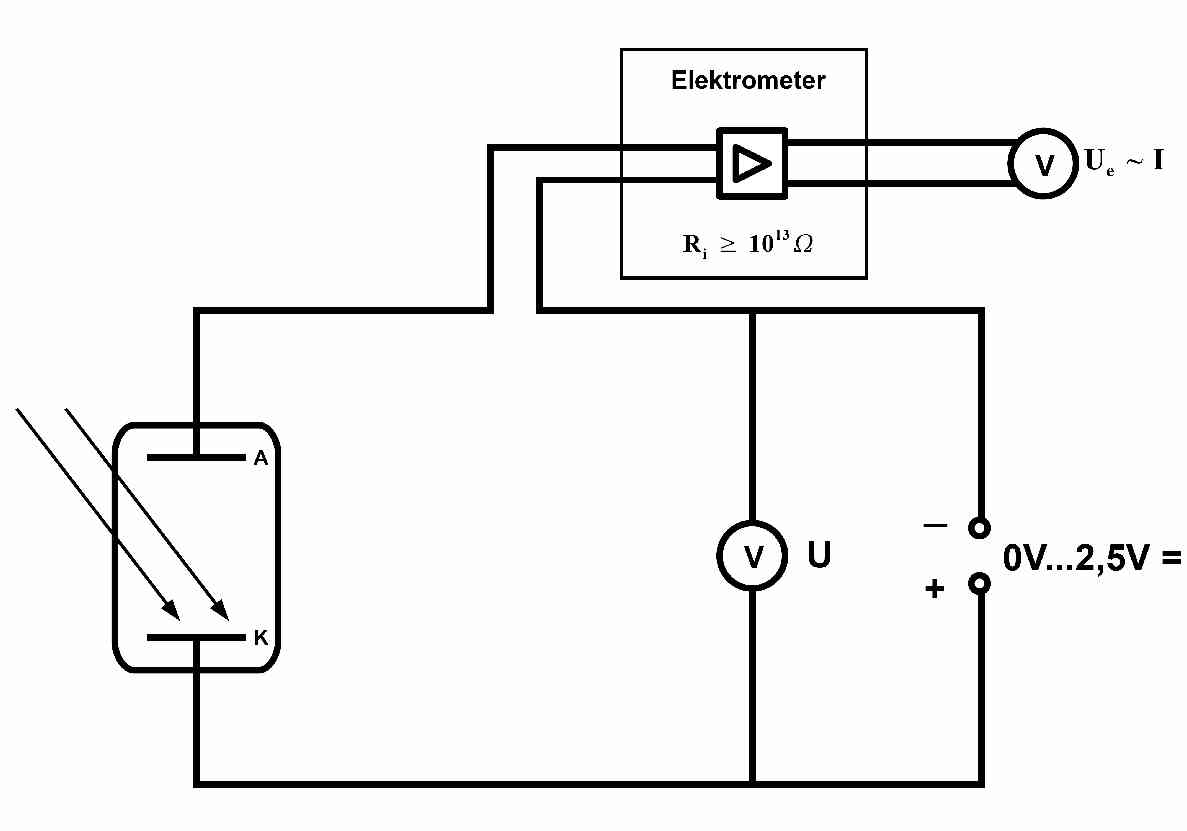
\includegraphics[width=0.7\textwidth]{../media/B1.4/Schaltplan_Gegenspannungsmethode.jpg}
	\caption{Schaltplan der Gegenspannungsmethode}
	\label{fig:Schaltplan Gegenspannungsmethode}
\end{figure}

\subsubsection{direkte Methode}
\label{durchführung:direkt}

Anstatt der Gegenspannung kann auch die Spannung an der Photozelle direkt gemessen werden. Dazu wird die Zelle mit dem Elektrometer verbunden. Wie bei der Gegenspannungsmethode ist der Messverstärker als ``Elektrometer'' eingestellt, der Innenwiederstand beträgt auch hier $10^{13}\,\Omega$.

Anders als bei der Gegenspannungsmethode muss die Photozelle bei der direkten Methode vor jeder Messung entladen werden, um die Spannung zurückzusetzen. Zu diesem Zweck besitzt sie einen Kurzschlussschalter.

\begin{figure}[h!]
	\centering
	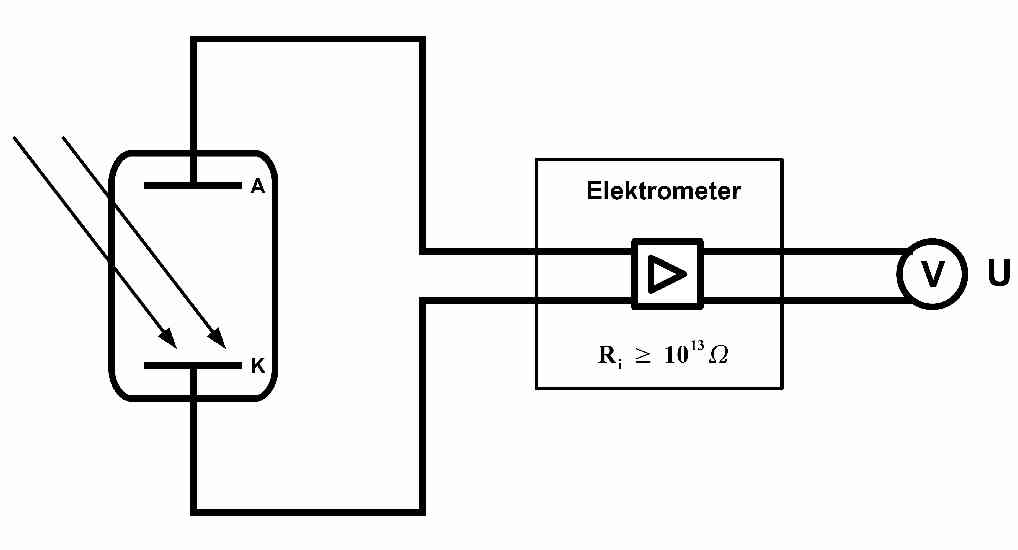
\includegraphics[width=0.7\textwidth]{../media/B1.4/Schaltplan_direkte_Methode.jpg}
	\caption{Schaltplan der direkten Methode}
	\label{fig:Schaltplan direkt}
\end{figure}

\subsection{Photostrom}

Zur Messung des Photostroms wird der Messverstärker auf ``Low Drift'' gestellt. Der Innenwiderstand wird auf $10\mathrm{\,k\Omega}$ heruntergeregelt, um einen Photostrom zu ermöglichen. Die Messung des Stroms erfolgt indirekt über eine Spannung, dazu wird ein Widerstand $R=10\mathrm{\,k\Omega}$ benutzt.

Die Zeitkonstante wird wie bei den vorherigen Messungen in Abschnitt \ref{durchführung:Energiemessung} als $0.3\mathrm{\,s}$ eingestellt, der Messverstärker dagegen auf $10^4$--fache Verstärkung erhöht. Da der Photostrom schwach ist, muss das Signal deutlich mehr verstärkt werden.

Für diesen Versuchsteil wird die \nameref{durchführung:direkt} verwendet, der Schaltplan ist in Abbildung \ref{fig:Schaltplan Photostrom} zu sehen. Die gemessene Spannung $U_e$ ist durch Ohm'sche Gesetz proportional zu dem Photostrom $I_\mathrm{Ph}$.

\begin{figure}[h!]
	\centering
	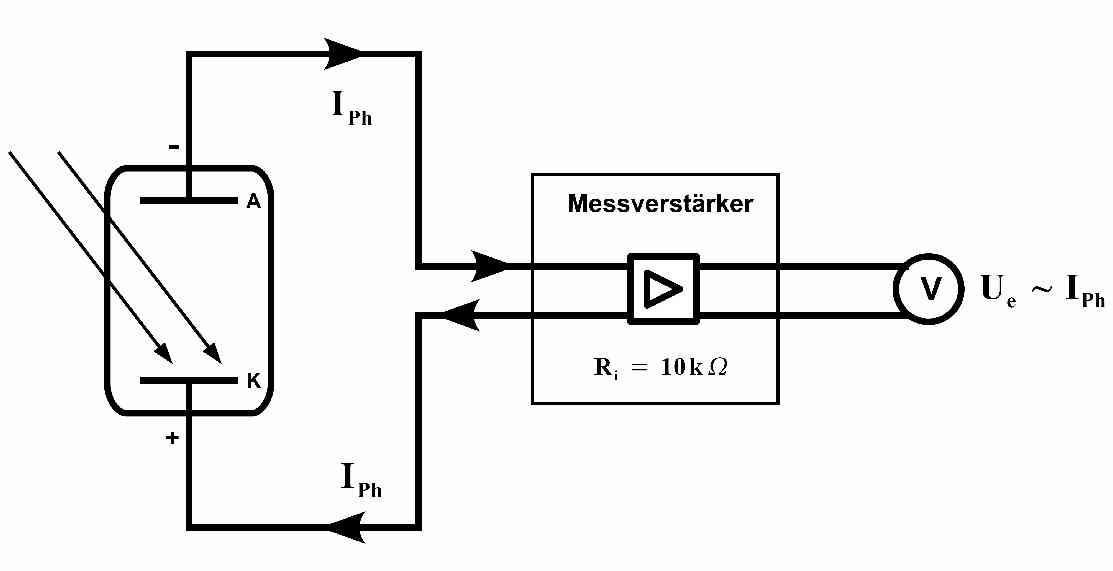
\includegraphics[width=0.7\textwidth]{../media/B1.4/Schaltplan_Photostrom.jpg}
	\caption{Schaltplan der Photostrommessung}
	\label{fig:Schaltplan Photostrom}
\end{figure}

\subsubsection{Photostrom}
Zur Messung des Photostroms werden abwechselnd der blaue und der grüne Interferenzfilter verwendet, zusammen mit einem von $6$ Graufiltern. Die Eigenschaften der Graufilter sind in Tabelle \ref{tab:Graufilter} dargestellt, die der Interferenzfilter in Tabelle \ref{tab:Interferenzfilter} in Abschnitt \ref{durchführung:Energiemessung}. Die Graufilter sind zwischen Interferenzfilter und Photozellengehäuse positioniert.

\begin{table}[h!]
	\centering
	\begin{tabular}{c|c|c|c|c|c|c}
		$\lambda$ $[\mathrm{nm}]$ & \multicolumn{6}{c}{Transmissionsgrad $T$ $[\%]$} \\
		& $1$ & $2$ & $3$ & $4$ & $5$ & $6$ \\
		\hline
		$436$ & $68$ & $48$ & $33$ & $28$ & $20$ & $14$ \\
		$546$ & $67$ & $46$ & $31$ & $23$ & $16$ & $11$
	\end{tabular}
	\caption{Eigenschaften der Graufilter mit $\Delta T=1\,\%$}
	\label{tab:Graufilter}
\end{table}

\subsubsection{Intensität}
Die direkte Messmethode aus Abschnitt \ref{durchführung:direkt} wird zudem dazu verwendet, die Abhängigkeit des Photostroms von der Intensität zu messen. Dabei wird die Stoppspannung mit dem grünen Interferenzfilter je einmal mit und ohne Graufilter $1$ gemessen. Dieser wird vor den Interferenzfilter gehalten, ohne befestigt zu werden.

\subsection{Leuchtdioden}

Zuletzt sollen die Wellenlängen von drei verschiedenen Leuchtdioden bestimmt werden.

Die jeweilige Leuchtdiode wird auf das Photozellengehäuse gesteckt und mit $I=100\mathrm{\,mA}$ betrieben. Dann wurde die Spannung mit der direkten Methode bestimmt, die in Abschnitt \ref{durchführung:direkt} beschrieben ist.

Für die Messungen werden Leuchtdioden mit den Farbbezeichnungen ``blue'', ``verde'' und ``true green'' verwendet. Der Schaltplan ist in Abbildung \ref{fig:Schaltplan LEDs} ersichtlich.

\begin{figure}[h!]
	\centering
	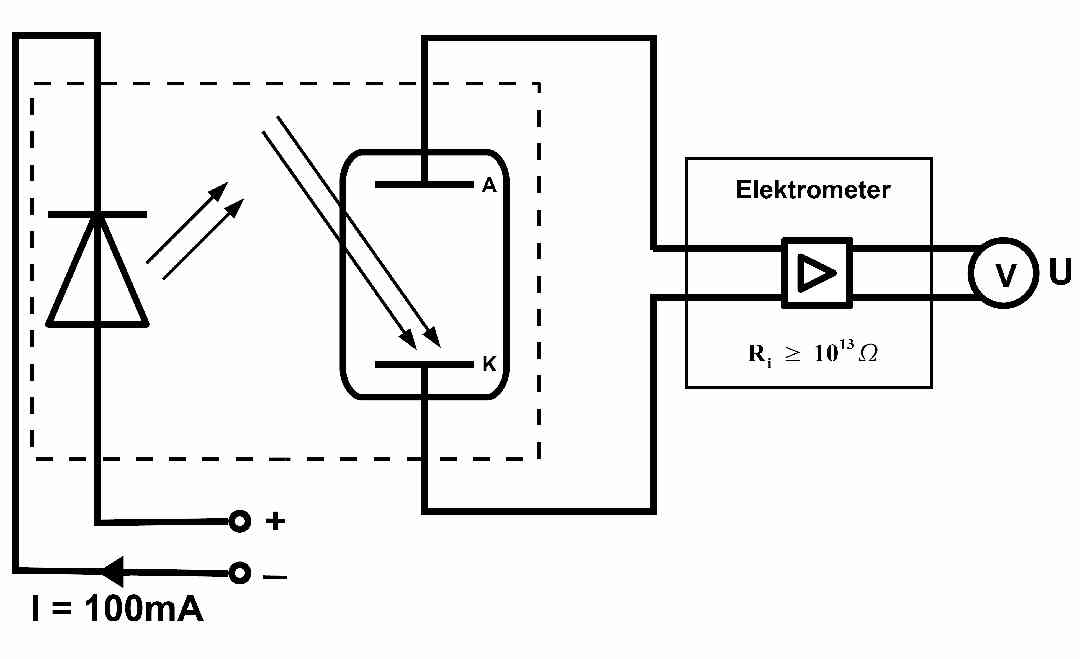
\includegraphics[width=0.7\textwidth]{../media/B1.4/Schaltplan_LED.jpg}
	\caption{Schaltplan der Messungen mit LEDs}
	\label{fig:Schaltplan LEDs}
\end{figure}


\clearpage
\hypertarget{auswertung}{\section{Auswertung}\label{auswertung}}
\subsection{Energie der Elektronen}
\label{auswertung:h/e}
Zunächst wird die Energie der Elektronen untersucht, woraus $\frac{h}{e}$ und die Austrittsarbeit der Anode $W_A$ bestimmt werden. Dies erfolgt für beide angewandte Messmethoden getrennt, womit die Ergebnisse verglichen werden können.

Dazu werden die Frequenzen $\nu$ zu den angegebenen Wellenlängen $\lambda$ bestimmt, wozu die Lichtgeschwindigkeit $c$ benötigt wird. Der Fehler $\Delta \nu$ folgt aus der Gauß'schen Fehlerfortpflanzung. Sie werden zusammen mit den Messergebnissen in Tabelle \ref{table:Messwerte Energie} dargestellt.

\begin{eqnarray}
	\nu &=& \frac{c}{\lambda} \label{eq:frequenzWellenlänge} \\
	\Delta \nu &=& \frac{c \cdot \Delta \lambda}{\lambda^2}
\end{eqnarray}

\begin{table}[h!]
	\centering
	\begin{tabular}{c|c|c|c|c}
		Messung & $\lambda$ [nm] & $\nu$ [$10^{14} \mathrm{\, Hz}$] & $U_{0,G}$ [V] & $U_{0,D}$ [V] \\
		\hline
		1 & $366 \pm 7$ & $8.19 \pm 0.16$ & $1.769 \pm 0.003$ & $1.770 \pm 0.003$ \\
		2 & $405 \pm 7$ & $7.40 \pm 0.13$ & $1.434 \pm 0.003$ & $1.434 \pm 0.003$ \\
		3 & $436 \pm 7$ & $6.88 \pm 0.11$ & $1.232 \pm 0.003$ & $1.232 \pm 0.003$ \\
		4 & $546 \pm 7$ & $5.49 \pm 0.07$ & $0.705 \pm 0.003$ & $0.696 \pm 0.003$ \\
		5 & $578 \pm 7$ & $5.19 \pm 0.06$ & $0.645 \pm 0.003$ & $0.635 \pm 0.003$
	\end{tabular}
	\caption{Gemessene Stoppspannungen nach Gegenspannungsmethode $U_{0,G}$ und direkter Methode $U_{0,D}$ zu Wellenlängen $\lambda$ bzw. Frequenzen $\nu$}
	\label{table:Messwerte Energie}
\end{table}

\begin{figure}[h!]
	\begin{minipage}{0.5\textwidth}
		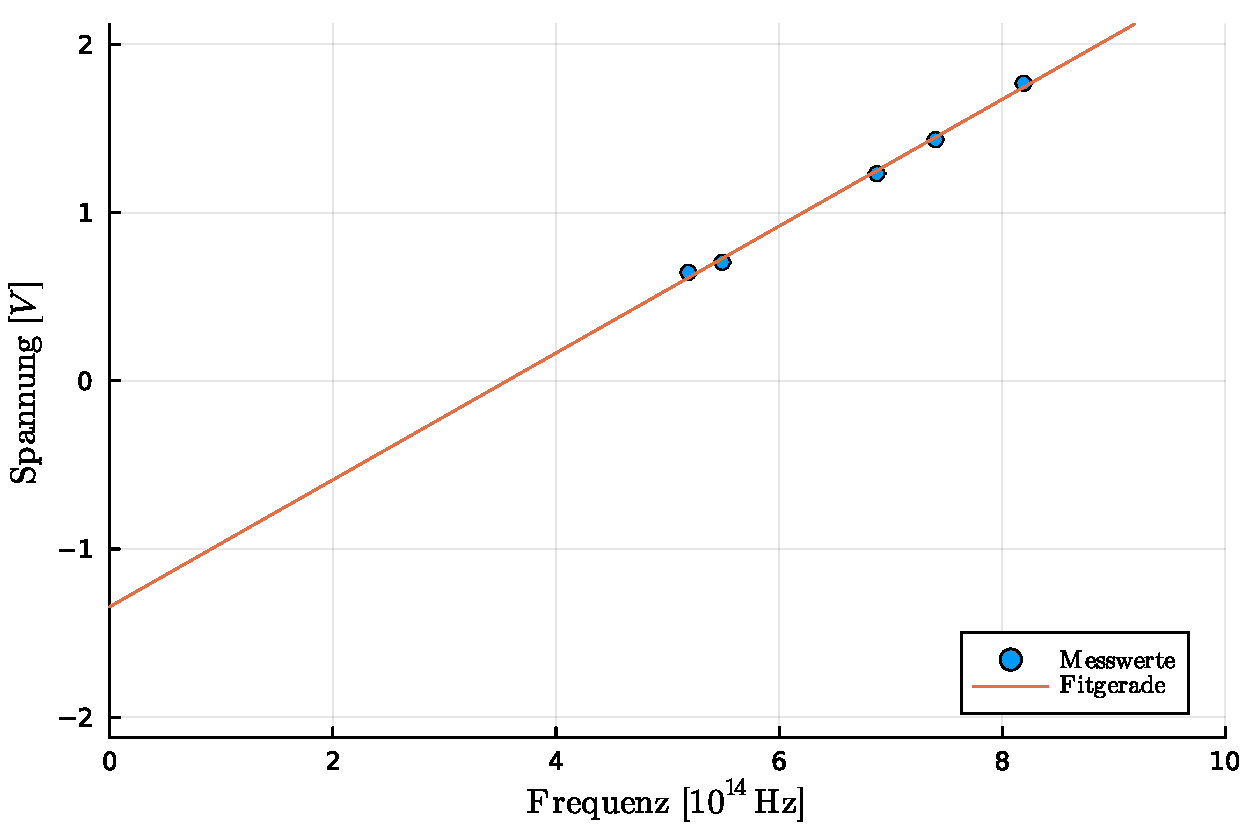
\includegraphics[width=\linewidth]{../media/B1.4/gegenPlot.pdf}
	\end{minipage}
	\begin{minipage}{0.5\textwidth}
		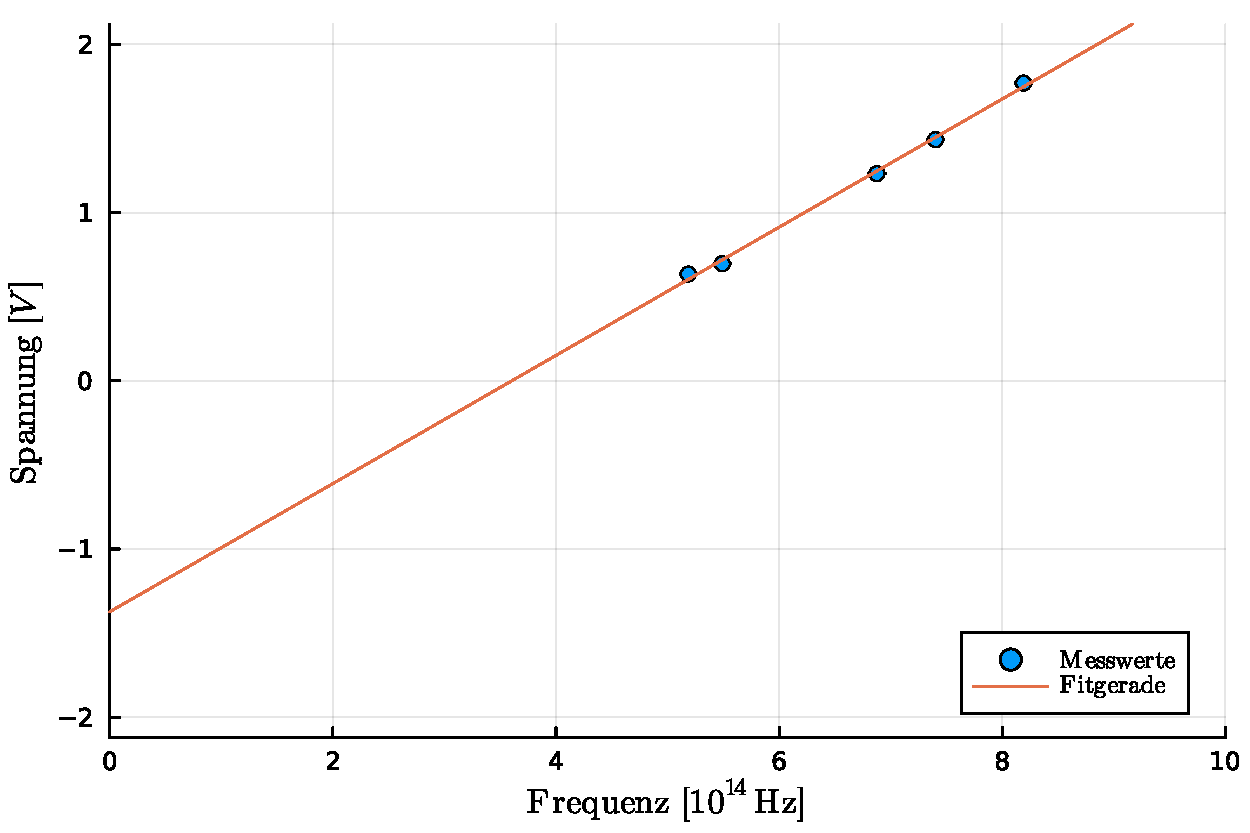
\includegraphics[width=\linewidth]{../media/B1.4/direktPlot.pdf}
	\end{minipage}
	\caption{Messwerte und Geradenanpassung aus der Gegenspannungsmethode (links) und der direkten Methode (rechts) \\
		Messfehler sind im Fit berücksichtigt, in der Darstellung aber nicht sichtbar}
	\label{fig:fitGeraden}
\end{figure}

\noindent
An diesen Ergebnissen wird mittels des \code{Julia}--Pakets \code{LsqFit} \cite{Julia:LsqFit} eine Geradenanpassung durchgeführt, die in Abbildung \ref{fig:fitGeraden} dargestellt ist.

Mithilfe von Gleichung \eqref{eq:Stoppspannung Geradengleichung} wird $\frac{h}{e}$ als Steigung $a$ identifiziert. Die Austrittsarbeit $W_A$ der Anode ergibt sich aus dem $y$--Achsenabschnitt $b$, wobei die Einheit Elektronenvolt vorausgesetzt ist. Die Ergebnisse sind in Tabelle \ref{table:Ergebnisse Energie} dargelegt.

\begin{eqnarray}
	\frac{h}{e} &=& a \label{eq:h/e Steigung} \\
	b &=& - \frac{W_A}{e} \label{eq:h/e Achsenabschnitt} \\
	\Leftrightarrow \quad W_A &=& - b \cdot e
\end{eqnarray}

\begin{table}[h!]
	\centering
	\begin{tabular}{l|c|c}
		& $\frac{h}{e}$ [$10^{-15} \mathrm{\, Vs}$] & $W_A$ $[\mathrm{eV}]$ \\
		\hline
		Gegenspannungsmethode & $3.77 \pm 0.11$ & $1.34 \pm 0.08$ \\
		direkte Methode & $3.81 \pm 0.11$ & $1.37 \pm 0.08$
	\end{tabular}
	\caption{Steigung $\frac{h}{e}$ und Austrittsarbeit $W_A$ der Anode}
	\label{table:Ergebnisse Energie}
\end{table}

\noindent
Die Austrittsarbeit $W_A$ kann alternativ aus der Nullstelle der gefitteten Geraden bestimmt werden kann. Dies wäre theoretisch eine genauere Methode der Bestimmung, da die Nullstelle näher als der $y$--Achsenabschnitt an den Messwerten liegt, damit wäre der Fehler geringer.

Allerdings ist die Nullstelle der Geraden nicht so genau bestimmbar wie der $y$--Achsenabschnitt, da letzterer direkt aus dem Fitprozess folgt. Die Nullstelle müsste dagegen extra ermittelt werden. Da sowohl Steigung als auch $y$--Achsenabschnitt fehlerbehaftet sind, würde der Fehler der Nullstelle durch die Fehlerfortpflanzung bestimmt werden müssen.

Die Bestimmung der Austrittsarbeit $W_A$ erfolgt durch den Achsenabschnitt, weil der Fehler der Nullstelle nur größer als der des Achsenabschnitts sein kann.

\subsubsection{Diskussion der Ergebnisse}
In der Literatur beträgt $\frac{h}{e}\approx4.14 \cdot 10^{-15} \mathrm{\, Vs}$. \cite{Gerthsen} Die Messergebnisse weichen auch innerhalb ihrer Fehler leicht von diesem Wert ab.

Dies könnte z.B. auf den Lichteinfall durch ein kleines Fenster und die Deckenlampen im Versuchsraum zurückzuführen sein, der die Messergebnisse möglicherweise verändert hat.

Die Größenordnung der ermittelten Austrittsarbeiten entsprechen den Erwartungen. Beispielsweise könnte die Kathode aus einer Wolfram--Cäsium--Legierung bestehen, deren Austrittsarbeit in der Größenordnung von $1.4\mathrm{\,eV}$ \cite{Demtröder} angegeben ist. Dieser Wert wird bei beiden Messmethoden innerhalb der Fehler getroffen.

Damit wird dieser Versuchsteil als Erfolg gewertet.

\subsubsection{Vergleich der Methoden}
Beide Messmethoden liefern die gleichen Ergebnisse innerhalb der Fehlergrenzen. Selbst die Ungenauigkeiten sind in den ersten Stellen gleich groß. Daher scheinen beide Methoden vergleichbar genau zu sein.

Vorteilhaft bei der Gegenspannungsmethode ist das Stoppen des Stromflusses durch die Gegenspannung. Fließt bei einer Spannungsmessung Strom, so wird diese beeinträchtigt. Somit liefert diese Methode eine ideale Spannungsmessung. Nachteilig ist die manuelle Einstellung der Gegenspannung, die aufgrund von starken Schwankungen ungenau ist.

Bei der direkten Messmethode muss dagegen keine ungenaue Gegenspannung eingestellt werden. Dies vereinfacht die Durchführung der Methode und reduziert eine Fehlerquelle. Dafür wird die Stoppspannung bei fließendem Strom gemessen. Auch wenn dieser eher klein ist, führt er dennoch zu einer systematischen Ungenauigkeit.

Obwohl die Gegenspannungsmethode theoretisch von Vorteil ist, sind beide Messmethoden in der Praxis vergleichbar genau. Falls die Gegenspannung digital ermittelt wird, könnte dies anders sein.

\subsection{Photostrom}
\subsubsection{Photostrom}

Der Photostrom $I_\mathrm{Ph}$ wird durch das Ohm'sche Gesetz aus der Photospannung $U_\mathrm{Ph}$ bestimmt. Der Widerstand in der Messung beträgt $10 \mathrm{\,k\Omega}$, die gemessene Spannung wurde um den Faktor $\alpha=10^4$ verstärkt. Die Ergebnisse sind in Tabelle \ref{tab:Photostrom Ergebnisse} dargestellt. Die Messung ohne Graufilter erfolgte, um ein Gefühl für den Strom bei $100\%$ Intensität zu erlangen.

\begin{eqnarray}
	I_\mathrm{Ph} &=& \frac{U_\mathrm{Ph}}{R \cdot \alpha} \\
	\Delta I_\mathrm{Ph} &=& \frac{\Delta U_\mathrm{Ph}}{R \cdot \alpha}
\end{eqnarray}

\begin{table}[h!]
	\centering
	\begin{tabular}{c|c|c|c|c|c|c|c|c}
		&& \multicolumn{7}{c}{Photostrom $I_\mathrm{Ph}$ $[10^{-8}\mathrm{\,A}]$} \\
		Filter & Farbe & $1$ & $2$ & $3$ & $4$ & $5$ & $6$ & ohne Filter\\
		\hline
		$3$ & Blau & $1.486$ & $1.067$ & $0.807$ & $0.655$ & $0.440$ & $0.338$ & $1.777$ \\
		$4$ & Grün & $0.536$ & $0.357$ & $0.265$ & $0.190$ & $0.126$ & $0.090$ & $0.608$
	\end{tabular}
	\caption{Photoströme für verschiedenen Graufilter mit $\Delta I_\mathrm{Ph} = \pm 5 \cdot 10^{-11} \mathrm{\,A}$}
	\label{tab:Photostrom Ergebnisse}
\end{table}

\noindent
Trägt man den Photostrom gegen die jeweiligen relativen Transmissionsgrade auf, erkennt man lineare Zusammenhänge, sichtbar in Abbildung \ref{abb:Photostrom fit}. Der Photostrom ist daher proportional zur Intensität der einfallenden Strahlung.

Auffällig sind die Unterschiede in der Stärke des Photostroms bei verschiedenen Farben. Der Photostrom ist bei Verwendung des blauen Interferenzfilters deutlich höher als bei der des grünen.

Das Phänomen kann durch die unterschiedliche Intensität im Linienspektrum von Quecksilber erklärt werden. Die Quecksilberdampflampe emittiert blaues Licht in höherer Intensität als grünes. Dadurch erreicht mehr Strahlung die Photokathode, da die transmittierte Intensität proportional zu der am Graufilter eintreffenden Intensität ist.

Die Fitfunktion bei beiden Filter besitzt einen endlichen Ordinatenabschnitt, der im Rahmen der Messungenauigkeit fast vollständig verschwindet. Bei einer Lichtintensität von $0$ gibt es keine Photonen, die Elektronen an der Kathode herauslösen können. Dadurch fließt kein Photostrom.

Ersichtlich ist eine starke Abweichung beider Photoströme für $100 \%$ Intensität, daher wurden diese Werte im Fit vernachlässigt. Zudem sollte dieser Wert ursprünglich nicht gemessen werden, sondern wurde nur aus Interesse ebenfalls aufgenommen.

\begin{figure}[h!]
	\begin{minipage}{0.5\textwidth}
		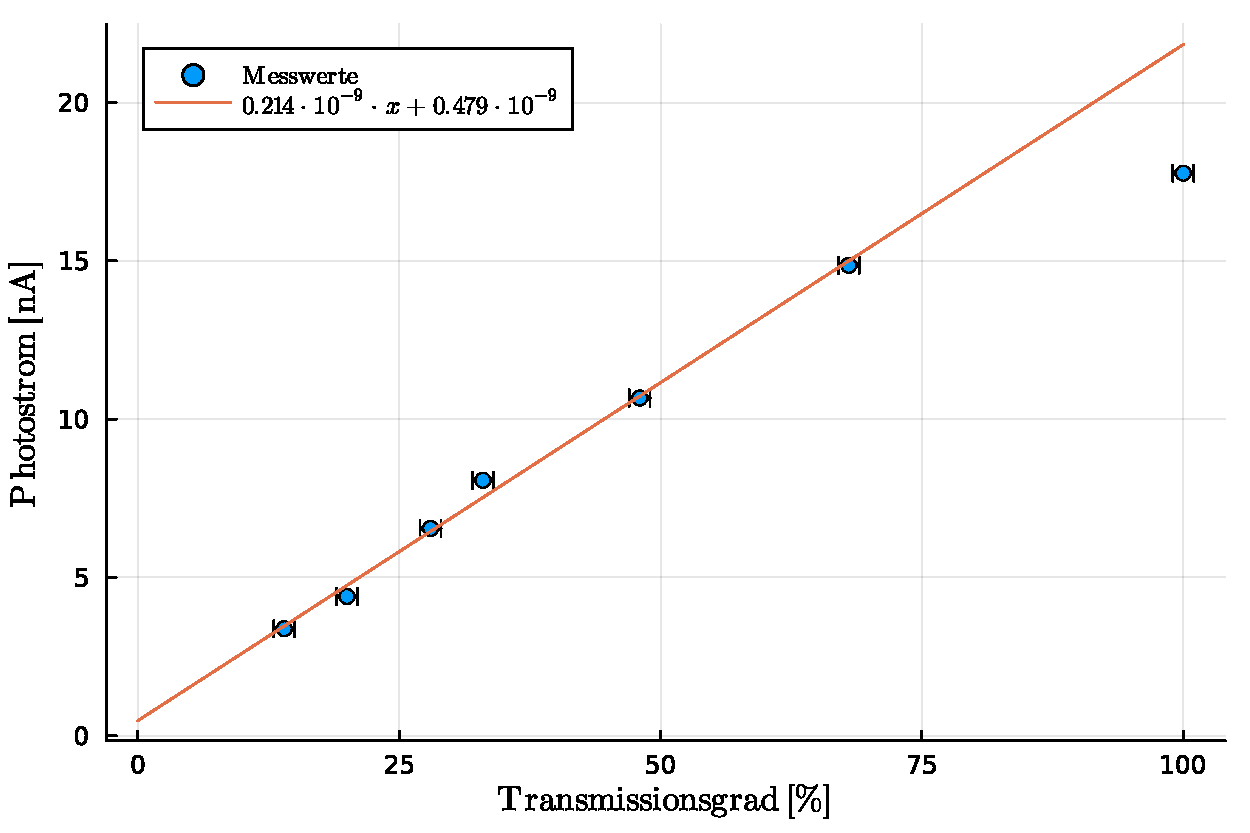
\includegraphics[width=\textwidth]{../media/B1.4/Photostrom_blau.pdf}
		\caption*{blauer Interferenzfilter}
		\label{abb:Photostrom blau}
	\end{minipage}
	\begin{minipage}{0.5\textwidth}
		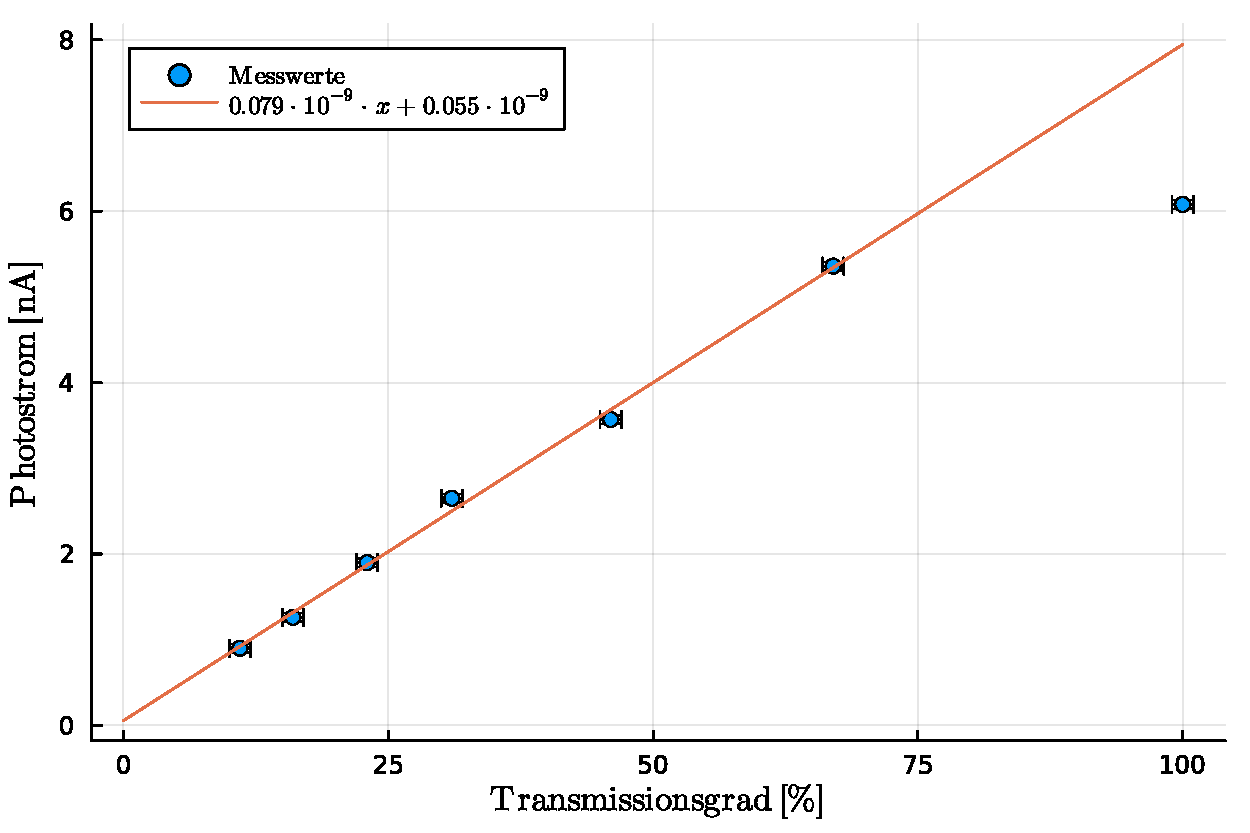
\includegraphics[width=\textwidth]{../media/B1.4/Photostrom_gruen.pdf}
		\caption*{grüner Interferenzfilter}
		\label{abb:Photostrom grün}
	\end{minipage}
	\caption{Photoströme bei verschiedenen Graufiltern}
	\label{abb:Photostrom fit}
\end{figure}


\subsubsection{Intensität}
Zusätzlich wird die Abhängigkeit der kinetischen Energie der Elektronen von der Lichtintensität untersucht. Dazu wird der stärkste Graufilter (Nummer $6$) vor die Lampe gehalten und die Veränderung der Stoppspannung beobachtet, die wie in Abschnitt \ref{auswertung:h/e} gemessen wird.

Die Ergebnisse zeigen deutlich die Unabhängigkeit dieser Größen und sind in Tabelle \ref{tab:Spannung Intensität} dargestellt. Innerhalb der Fehler sind die Spannungen identisch, obwohl der Intensitätsunterschied ziemlich groß ist.

Eine höhere Intensität entspricht einer größere Photonendichte. Die Anzahl der Photonen ist jedoch irrelvant für die Energie der ausgelösten Elektronen. Nach der klassischen Wellentheorie bekämen die Elektronen durch höhere Intensität mehr Energie, was hier eindeutig nicht zu beobachten ist. Daher belegen die Messungen die Quantenhypothese für Licht.

\begin{table}[h!]
	\centering
	\begin{tabular}{l|c}
		& Stoppspannung $[\mathrm{V}]$ \\
		\hline
		ohne Graufilter & $0.688 \pm 0.005$ \\
		Graufilter $6$ & $0.693 \pm 0.005$
	\end{tabular}
	\caption{Spannung bei verschiedenen Intensitäten}
	\label{tab:Spannung Intensität}
\end{table}

\subsection{Untersuchung von Leuchtdioden mit der Photozelle}

Zuletzt werden die Wellenlängen von drei Leuchtdioden aus gemessenen Stoppspannungen bestimmt. Zur Messung wurde die direkte Methode verwendet, weshalb im Folgenden die Messergebnisse ebendieser Methodik gewählt werden..

In Abschnitt \ref{auswertung:h/e} wurde anhand der Messergebnisse eine Geradengleichung ermittelt, die im Folgenden verwendet wird. Sie ergibt sich aus den Gleichungen \eqref{eq:h/e Steigung} und \eqref{eq:h/e Achsenabschnitt} sowie den Werten aus Tabelle \ref{table:Ergebnisse Energie}. Hierbei wird die Austrittsarbeit durch die Elementarladung $\mathrm{e}$ dividiert.

\begin{eqnarray}
	U_0 &=& a \cdot \nu + b \\
	a &=& (3.81\pm 0.11)\cdot10^{-15}\mathrm{\,Vs} \\
	b &=& (1.37 \pm 0.08) \,\frac{\mathrm{eV}}{\mathrm{e}}
\end{eqnarray}

\noindent
Die Umformung dieser Gleichung ermöglicht die Bestimmung der Wellenlängen $\lambda$ aus den gemessenen Stoppspannungen $U_0$, wobei Gleichung \eqref{eq:frequenzWellenlänge} mit der Lichtgeschwindigkeit $c$ Anwendung findet. Der Fehler $\Delta \lambda$ folgt nach Gauß'scher Fehlerfortpflanzung.

\begin{eqnarray}
	\lambda &=& \frac{a \cdot c}{U_0 - b} \\
	\Delta \lambda &=&
		\sqrt{
			\left(
				\frac{c \cdot \Delta a}{U_0 - b}
			\right)^2
			+ \left(
				\frac{a \cdot c \cdot \Delta U_0}{(U_0 - b)^2}
			\right)^2
			+ \left(
				\frac{a \cdot c \cdot \Delta b}{(U_0 - b)^2}
			\right)^2
		}
\end{eqnarray}

\noindent
Üblicherweise senden Leuchtdioden ein Spektrum von Licht aus, anstelle von monochromatischem Licht. In diesem Versuch wurde allerdings nur eine Wellenlänge pro Leuchtdiode bestimmt.

Bei der Messung der Stoppspannung wird die maximale Energie gemessen, die ein ausgelöstes Elektron erhalten kann. Die schnellsten Elektronen werden durch die Photonen mit maximaler Energie erzeugt, also durch die mit der niedrigsten verfügbaren Wellenlänge.

Die hier bestimmte Wellenlänge $\lambda$ ist daher die niedrigste Wellenlänge des jeweiligen LED--Spektrums. Üblicherweise ist ein solches Spektrum näherungsweise gaußverteilt. Damit liegen die Mittelwerte der Verteilungen bei einer größeren Wellenlänge als der hier bestimmten.

Das Intervall $[\mu - 3 \sigma, \mu + 3 \sigma]$ umfasst ca. $99.7 \mathrm{\, \%}$ der enthaltenen Werte einer Gaußverteilung, wobei $\mu$ der Mittelwert und $\sigma$ die Standardabweichung der Verteilung sind. \cite{LambacherSchweizerGauß} Daher liegen die gemessenen minimalen Wellenlängen ca. $3 \sigma$ vom Mittelwert $\mu$ entfernt. Die Halbwertsbreite $\sigma_\mathrm{FWHM}$ der Verteilungen der Leuchtdioden beträgt etwa $30 \mathrm{\, nm}$ \cite{uni}. Daher wird hier der Wert $\sigma_\mathrm{FWHM}=(30\pm0.5)\mathrm{\,nm}$ angenommen.

Die Standardabweichung $\sigma$ lässt daher mittels der Gleichungen \eqref{eq:halbwertsbreite} \cite{Halbwertsbreite} und \eqref{eq:halbwertsbreiteFehler} bestimmen, der Mittelwert $\mu$ durch \eqref{eq:mittelwertLEDs} und \eqref{eq:mittelwertLEDsFehler}. Die Fehler folgen aus der Gauß'schen Fehlerfortpflanzung.

Die Ergebnisse sind in Tabelle \ref{table:leds} dargestellt.


\begin{eqnarray}
	\sigma_\mathrm{FWHM} &=& 2 \sqrt{2 \ln{2}} \cdot \sigma
		\label{eq:halbwertsbreite} \\
	\Delta \sigma &=& \frac{\Delta \sigma_\mathrm{FWHM}}{2 \sqrt{2 \ln{2}}}
		\label{eq:halbwertsbreiteFehler} \\
	\mu &=& \lambda + 3 \sigma
		\label{eq:mittelwertLEDs} \\
	\Delta \mu &=& \sqrt{\left(\Delta \lambda\right)^2 + \left(3 \cdot \Delta \sigma \right)^2}
		\label{eq:mittelwertLEDsFehler}
\end{eqnarray}

\begin{table}[h!]
	\centering
	\begin{tabular}{l|c|c|c|c|c}
		Bezeichnung & $U_0$ $[\mathrm{V}]$ & $\lambda$ $[\mathrm{nm}]$ & $\sigma$ $[\mathrm{nm}]$ & $\mu$ $[\mathrm{nm}]$ & Literaturwert $[\mathrm{nm}]$ \\
		\hline
		blue & $1.047 \pm 0.003$ & $472 \pm 20$ & $12.74 \pm 0.21$ & $510 \pm 20$ & $400 - 490$ \\
		verde & $0.891 \pm 0.003$ & $504 \pm 22$ & $12.74 \pm 0.21$ & $542 \pm 22$ & $490 - 570$ \\
		true green & $0.807 \pm 0.003$ & $524 \pm 24$ & $12.74 \pm 0.21$ & $562 \pm 24$ & $490 - 570$
	\end{tabular}
	\caption{Gemessene Stoppspannungen $U_0$, berechnete Wellenlängen $\lambda$, Standardabweichungen $\sigma$, Mittelwerte $\mu$ und~Literaturwerte~\cite{Gerthsen}}
	\label{table:leds}
\end{table}

\noindent
Alle gemessenen minimalen Wellenlängen, sowie die daraus bestimmten Mittelwerte der Verteilungen liegen innerhalb ihrer Fehlergrenzen in den jeweiligen Bereichen der Literaturwerte, deshalb kann dieser Versuchsteil als erfolgreich betrachtet werden.

\clearpage
\hypertarget{fazit}{%
\section{Fazit}\label{fazit}}
Die in diesem Versuch gewonnenen Ergebnisse bestätigen die theoretischen Grundlagen des äußeren Photoeffekts. Die durchgeführten Experimente demonstrieren die Abhängigkeit der kinetischen Energie der ausgestoßenen Elektronen von der Frequenz des einfallenden Lichts sowie ihre Unabhängigkeit von dessen Intensität. Dieser Zusammenhang unterstützt die Quantenhypothese für Licht.

Die Messung von $\frac{h}{e}$ liefert ein grob vergleichbares, aber von der Literatur abweichendes Ergebnis. Die Messungen der Austrittsarbeit zeigen eine gute Übereinstimmung mit den theoretischen Werten, obwohl kleinere Abweichungen aufgrund externer Faktoren wie Umgebungslicht und den Materialeigenschaften der Elektroden auftreten. Beide verwendeten Messmethoden liefern innerhalb der Fehlergrenzen vergleichbare Ergebnisse. Jede Methode hat spezifische Vor- und Nachteile: Während die direkte Messmethode einfacher und präziser durchzuführen ist, könnte die Gegenspannungsmethode theoretisch präzisere Ergebnisse ermöglichen.

Die Experimente zur Untersuchung des Zusammenhangs zwischen Photostrom und Lichtintensität bestätigten die Proportionalität dieser Größen. Unterschiede im Photostrom bei verschiedenen Lichtfarben gehen auf die Intensität der jeweiligen Farblinien im Emissionsspektrum der Lichtquelle zurück.

Die Messung der minimalen Wellenlängen des Lichts, das von Leuchtdioden emittiert wurde, entspricht den Literaturwerten und bestätigt die korrekte Durchführung der Versuche.

Zusammenfassend bestätigen die Ergebnisse die Quantenhypothese für Licht und den photoelektrischen Effekt. Trotz kleiner systematischer Fehler und externer Einflüsse kann die theoretische Erwartung gut nachvollzogen werden. Somit gelten die Experimente als erfolgreich durchgeführt.

\clearpage
\hypertarget{literatur}{%
\section{Literatur}\label{literatur}}
\renewcommand{\section}[2]{}

\begin{thebibliography}{99}
\bibitem{Demtröder}
	W. Demtröder, ``Experimentalphysik 3'', $5.$ Auflage, Springer Verlag,
	DOI~\href{https://doi.org/10.1007/978-3-662-49094-5}{10.1007/978-3-662-49094-5}
\bibitem{Gerthsen}
	D. Meschede, ``Gerthsen Physik'', $25.$ Auflage, Springer Verlag,
	DOI~\href{https://doi.org/10.1007/978-3-662-45977-5}{10.1007/978-3-662-45977-5}
\bibitem{uni}
	Universität zu Köln, ``B1.4: Photoeffekt: Bestimmung von $h/e$'', Juli 2008,
	Online verfügbar unter \url{https://teaching.astro.uni-koeln.de/sites/default/files/praktikum_b/Anleitung_1.4.pdf},
	Abruf am 10.04.2024
\bibitem{Julia:LsqFit}
	\code{\href{https://julialang.org}{Julia}}--Paket \code{LsqFit},
	Dokumentation unter \url{https://docs.juliahub.com/General/LsqFit/stable}
\bibitem{LambacherSchweizerGauß}
	Rebecca Roy, ``Lambacher Schweizer Kursstufe'', Klett Verlag, 2020, ISBN 978-3-12-735310-5, Ausschnittsweise online verfügbar unter \url{https://www.klett.de/inhalt/media_fast_path/32/735310_Stochastik_Normalverteilung_und_Sigma_Regeln.pdf},
	Abruf 18.07.2024
\bibitem{Halbwertsbreite}
	Wikipedia, ``Halbwertsbreite'', \url{https://de.wikipedia.org/wiki/Halbwertsbreite}, Abruf am 18.07.2024
\end{thebibliography}
\end{document}
